\documentclass{article}
\usepackage[a0paper,margin=3cm]{geometry} % A0にしつつ余白なし
\usepackage[utf8]{inputenc}
\usepackage{graphicx} % 画像のため
\usepackage{multicol} % 複数カラム
\usepackage{xcolor} % 色の設定
\usepackage{tcolorbox}
\usepackage{lmodern}  % 欧文フォントを適切に扱う
\geometry{papersize={90cm,120cm}} % ポスターサイズを設定

\begin{document}

\begin{center}
{\fontsize{80}{90}\selectfont \bfseries 画像処理と次数制約付き最小全域木に基づく}\\
\vspace{1cm}
{\fontsize{80}{90}\selectfont \bfseries 細胞系統擬似時間の予測手法の改良}\\
\vspace{1cm}
{\fontsize{50}{50}\selectfont \bfseries 阿久津研究室　岩城拓磨}
\end{center}

\vspace{1cm}
\begin{multicols}{2}
\section*{\fontsize{60}{0}\selectfont 梗概}
\section*{\fontsize{60}{0}\selectfont ENGLISH}

\begin{minipage}{\columnwidth}
\vspace{1cm}
\baselineskip=43pt 
{\fontsize{35}{100}\selectfont シングルセルRNAシーケンシングは、細胞1つ1つの遺伝子発現情報を計測することができる。細胞の遺伝


データ解析を通じて生物学的プロセスにおける変化の連続性を再構築 することが可能である。細胞系統擬似時間解析のためのツールとして Slingshot や Monocle が広く利用されており、これらは最小全域木を用いて生物学的プロ セスの軌道を予測している。しかし、これらのツールは「細胞の状態が一度に 3 つ以上には遷移しない」という生物学的前提を考慮していない。本研究では、 Slingshot を改良し、この課題を解決した。また Slingshot では入力データをク ラスタリングする必要があるが、適切なクラスタ方法やパラメータの決定方法 などは不明である。画像処理によってクラスタ時に使用するパラメータを自動 決定することでこの課題を解決した。具体的には次の方法で解析を行う。2 次 元に次元削減後の シングルセル RNA シーケンシングデータをヒストグラムを 用いて画像として認識する。その画像に対して細線化処理をすることで大まか な木構造を計算する。その木構造の分岐と葉の数を調べることでシングルセル RNA シーケンシングデータのクラスタ数を決定する。シングルセル RNA シー ケンシングデータをクラスタリングしその重心と決定したクラスタ数を用いて 次数制限付き最小全域木を構築することで、「細胞の状態が一度に 3 つ以上には 遷移しない」という生物学的前提を考慮した細胞状態の遷移構造とする。得られ た最小全域木を principal curve で曲線にフィッティングすることで細胞系統擬 似時間の軌道とする。この改良の有効性は、Bone marrow mononuclear cell、 Hematopoiesis、Human fetal immune cell、および C. elegans の公開データ セットを用いて実証した。}
\end{minipage}
\vspace{1cm}
\section*{\fontsize{60}{0}\selectfont 擬似時間解析}
\begin{minipage}{\columnwidth}
\begin{tcolorbox}[colframe=black!70, colback=white, boxrule=0.2mm, width=\columnwidth, arc=2mm]
  \begin{center}
    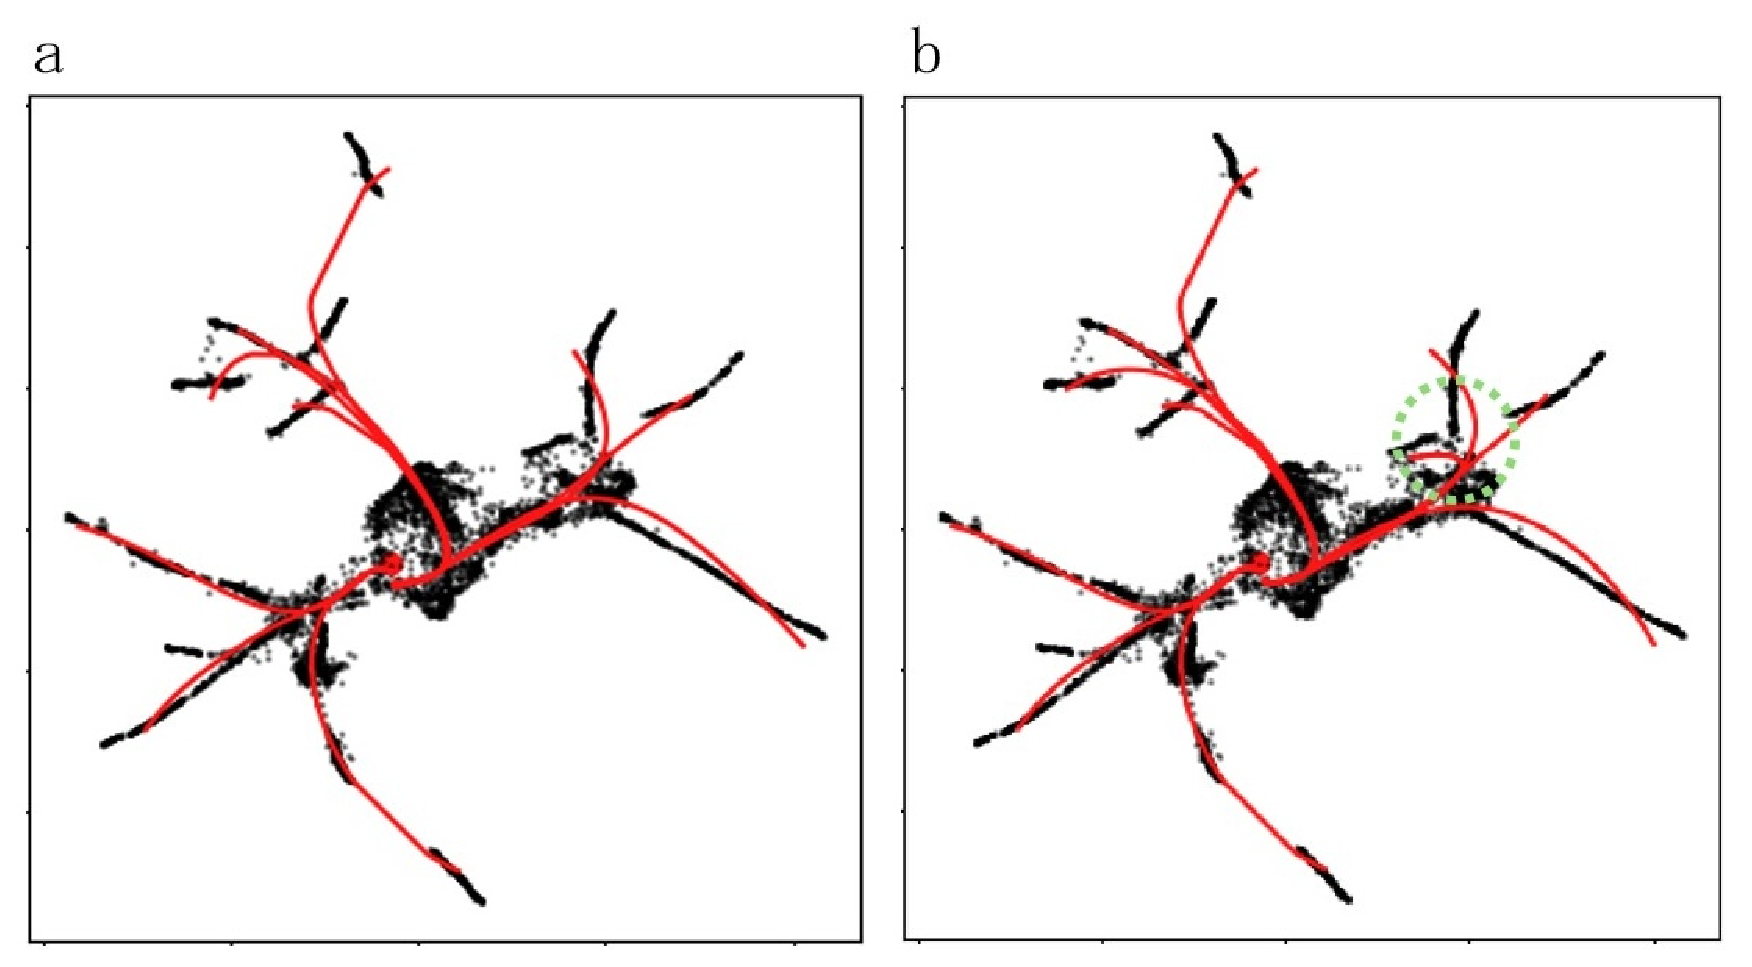
\includegraphics[width=0.66\columnwidth]{./img/Slide10.eps}
    
\includegraphics[width=0.33\columnwidth]{./img/Slide24.eps}
  \end{center}

{\fontsize{35}{35}\selectfont \textbf{図13:} クラスタ数による最小全域木の比較図。Hematopo}
\end{tcolorbox}

\end{minipage}
%\hspace{1cm}

%\hspace{1cm}


\vspace{1cm} %\\\vspace{-10cm}
\section*{\fontsize{60}{0}\selectfont 擬似時間解析}
\section*{\fontsize{60}{0}\selectfont Slingshot}
  
\vspace{1cm}
%\hspace{1cm}
\begin{minipage}{\columnwidth}
\begin{tcolorbox}[colframe=black!70, colback=white, boxrule=0.2mm, width=\columnwidth, arc=2mm]
  \begin{center}
    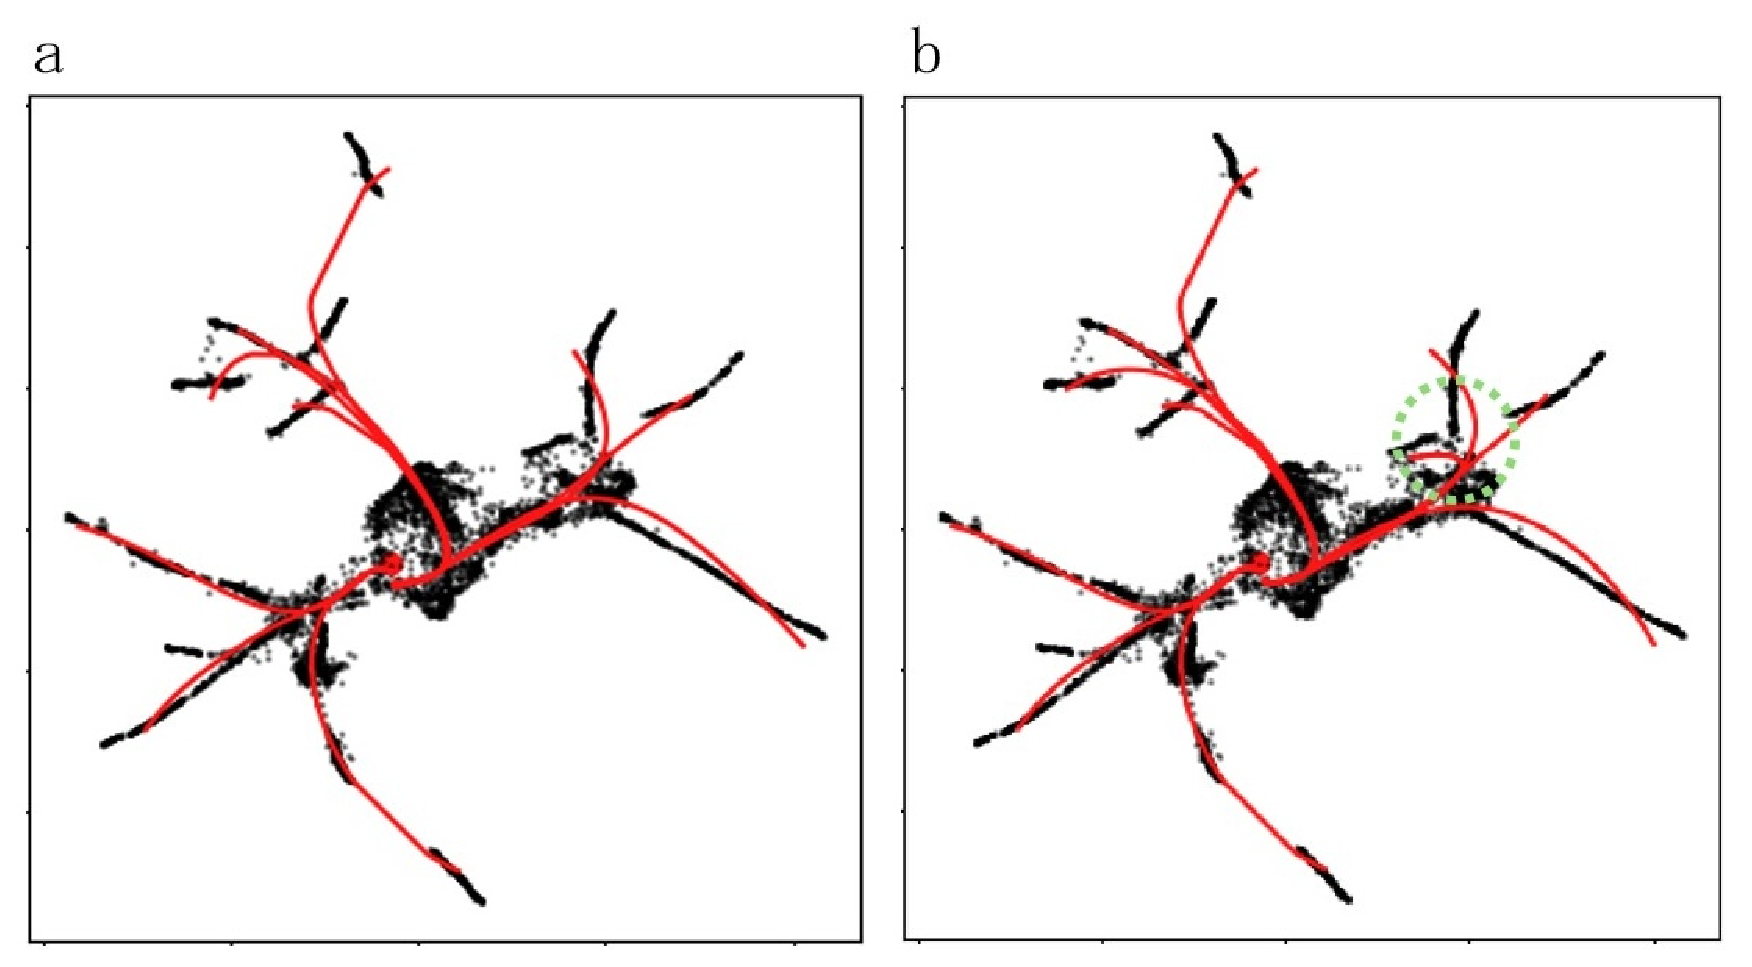
\includegraphics[width=0.66\columnwidth]{./img/Slide10.eps}
    
\includegraphics[width=0.33\columnwidth]{./img/Slide24.eps}
  \end{center}

{\fontsize{35}{35}\selectfont \textbf{図13:} クラスタ数による最小全域木の比較図。Hematopo}
\end{tcolorbox}
\end{minipage}
%\hspace{1cm}
\vspace{1cm} %\\\vspace{-10cm}
\section*{\fontsize{60}{60}\selectfont 次数制約付最小全域木}
\vspace{1cm}
%\hspace{1cm}
\begin{minipage}{\columnwidth}
\begin{tcolorbox}[colframe=black!70, colback=white, boxrule=0.2mm, width=\columnwidth, arc=2mm]
  \begin{center}
    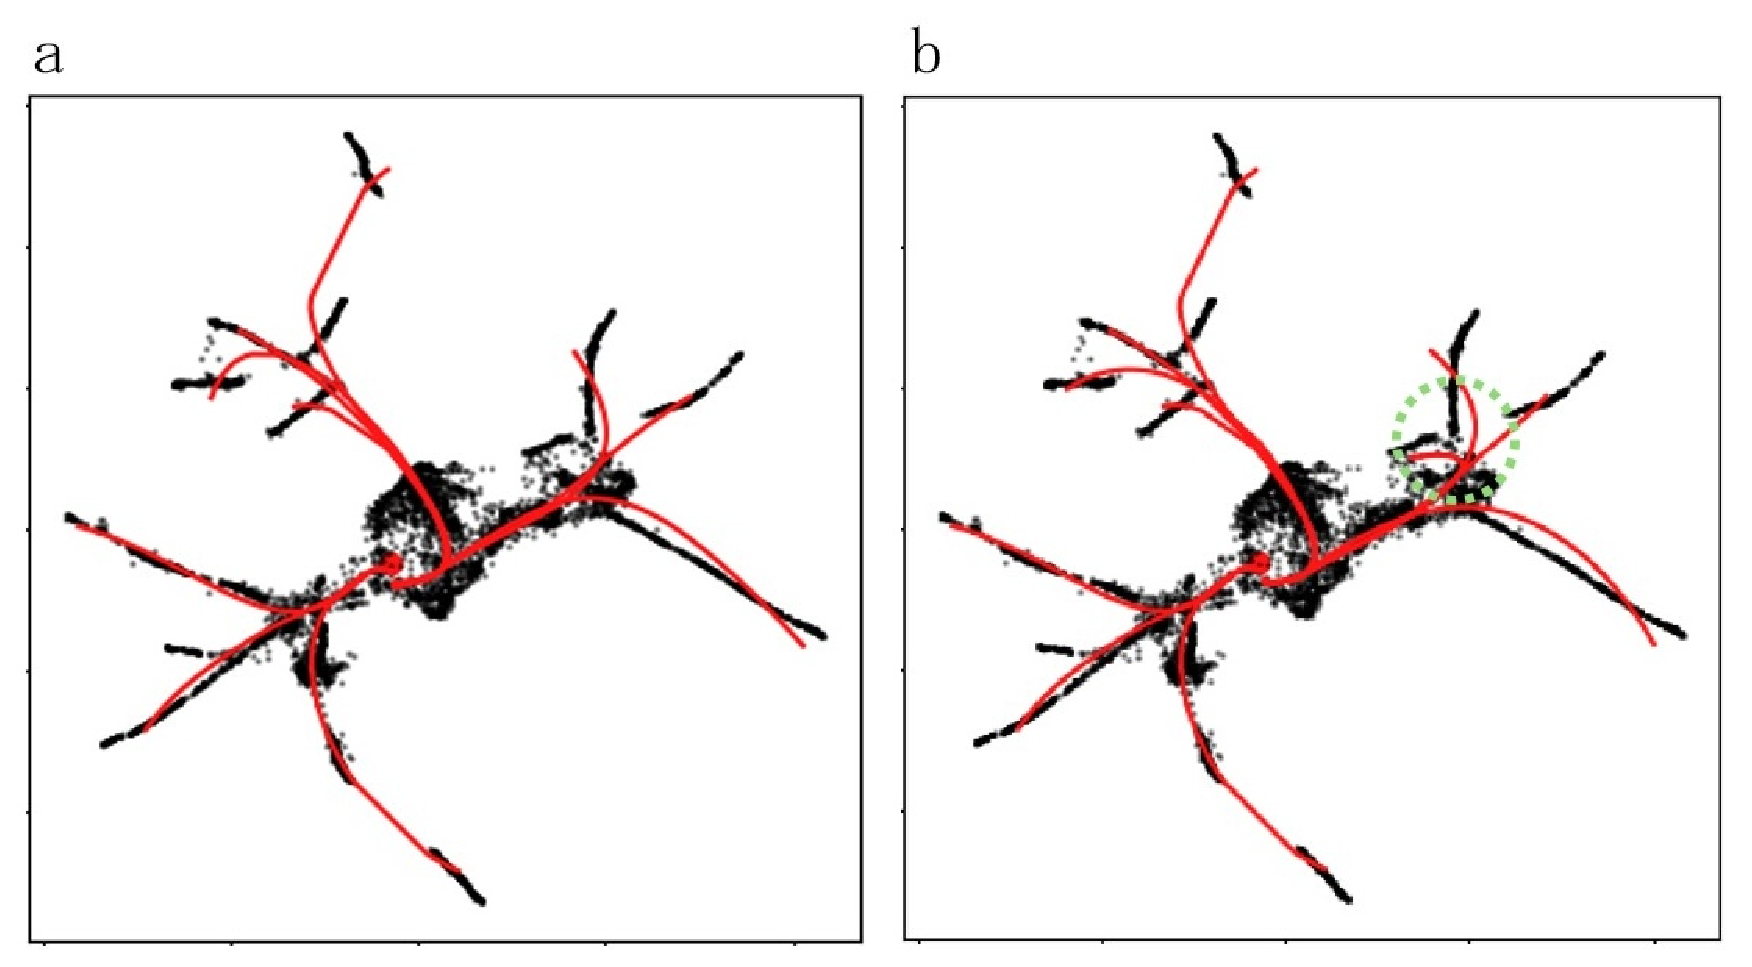
\includegraphics[width=0.66\columnwidth]{./img/Slide10.eps}
    
\includegraphics[width=0.33\columnwidth]{./img/Slide24.eps}
  \end{center}

{\fontsize{35}{35}\selectfont \textbf{図13:} クラスタ数による最小全域木の比較図。Hematopo}
\end{tcolorbox}
\end{minipage}
\vspace{1cm} %\\\vspace{-10cm}
\section*{\fontsize{60}{60}\selectfont 結果}
\vspace{1cm}
{\fontsize{35}{35}\selectfont 本文本文本文本文本文本文本文本文本文本文本文本文本文本文本文本文本文本文本文本文本文本文本文本文本文本文本文本文本文本文本文本文本文本文本文}
%\hspace{1cm}
\begin{tcolorbox}[colframe=black!70, colback=white, boxrule=0.2mm, width=\columnwidth, arc=2mm]
  \begin{center}
    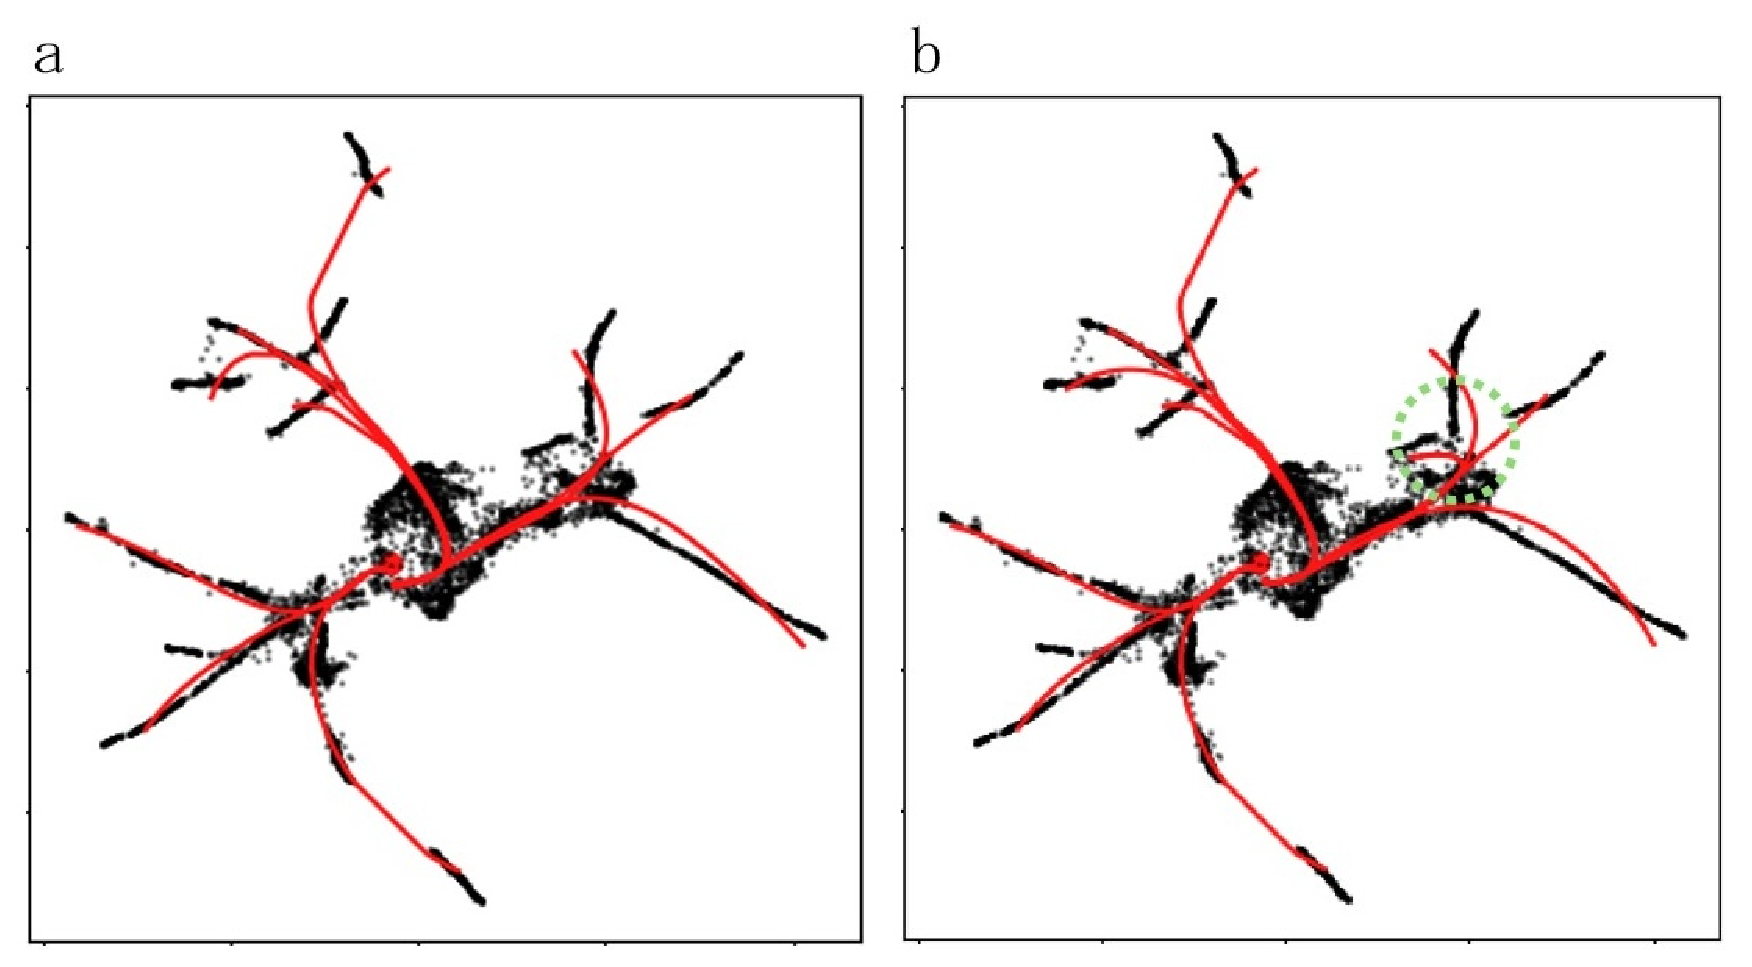
\includegraphics[width=0.66\columnwidth]{./img/Slide10.eps}
    
\includegraphics[width=0.33\columnwidth]{./img/Slide24.eps}
  \end{center}

{\fontsize{35}{35}\selectfont \textbf{図13:} クラスタ数による最小全域木の比較図。Hematopoiesisのデータを使用している。}
\end{tcolorbox}



\end{multicols}

\end{document}
